Nach dem Start der App muss dem \gls{spieler} das Hauptmenü angezeigt werden.
Von dort aus muss er die folgenden Möglichkeiten haben:
\begin{itemize}
    \item einen Button zum Starten eines neuen Spiel
    \item einen Button für bereits erreichte Highscores
    \item einen Button zum Einsehen und Nutzen des Stores
    \item einen Button zum Einsehen der Credits
\end{itemize}

Ein Button zur Sprachauswahl wird allerdings als \gls{niceToHave} betrachtet.
\\
Im Folgenden werden die einzelnen Anforderungen weiter erläutert:

Der \gls{spieler} muss in der Lage sein, den Screen zum Erstellen und Starten eines neuen Spiels zu erreichen. Auf diesem
Screen muss der Nutzer den Spielmodus auswählen. Dem Nutzer muss es danach möglich sein die Schwierigkeit auszuwählen.
Startet der Nutzer das von ihm erstellte Spiel, muss er direkt auf das Spielfeld kommen und das von ihm gewählte Spiel starten zu können.

Möchte der Nutzer das Spiel pausieren, so ist das mit einem Pause-Button möglich, welcher oben rechts auf dem Bildschirms plaziert sein muss.
Ist für einen \gls{spieler} das Spiel aus(keine Leben übrig), so muss er einmalig die Möglichkeit haben, optional durch die Anzeige eines Werbungsvideos, ein weiteres Leben zu bekommen und weiter zu spielen.
Ist ein Spieldurchlauf beendet und der erreichte Score ist in den Top 10 der Highscore, so muss der Nutzer die Möglichkeit haben seinen Namen zu dem erreichten Score einzutragen.

Entscheidet sich der Nutzer dazu, bereits erreichte Highscores einzusehen, muss er in der Lage sein einen durch einen Button, die lokalen Highscores einzusehen.

Möchte der \gls{spieler} den Store durchsuchen und/oder neue skin auswählen, muss er diesen Bereich ebenfalls von dem Hauptmenü aus erreichen. 
Im Store muss es dem Nutzer möglich sein aus einem von mindestens fünf skins für seinen ball und dessen Schweif, balken und Spiel-Hintergrund auszuwählen.

Um die Credits der "PONG" App einzusehen muss es dem Nutzer möglich sein von dem Hauptmenü aus einen Credits-Screen zu erreichen. Dort findet er Entwickler und anderweitig beteiligte Personen.

\begin{figure}
    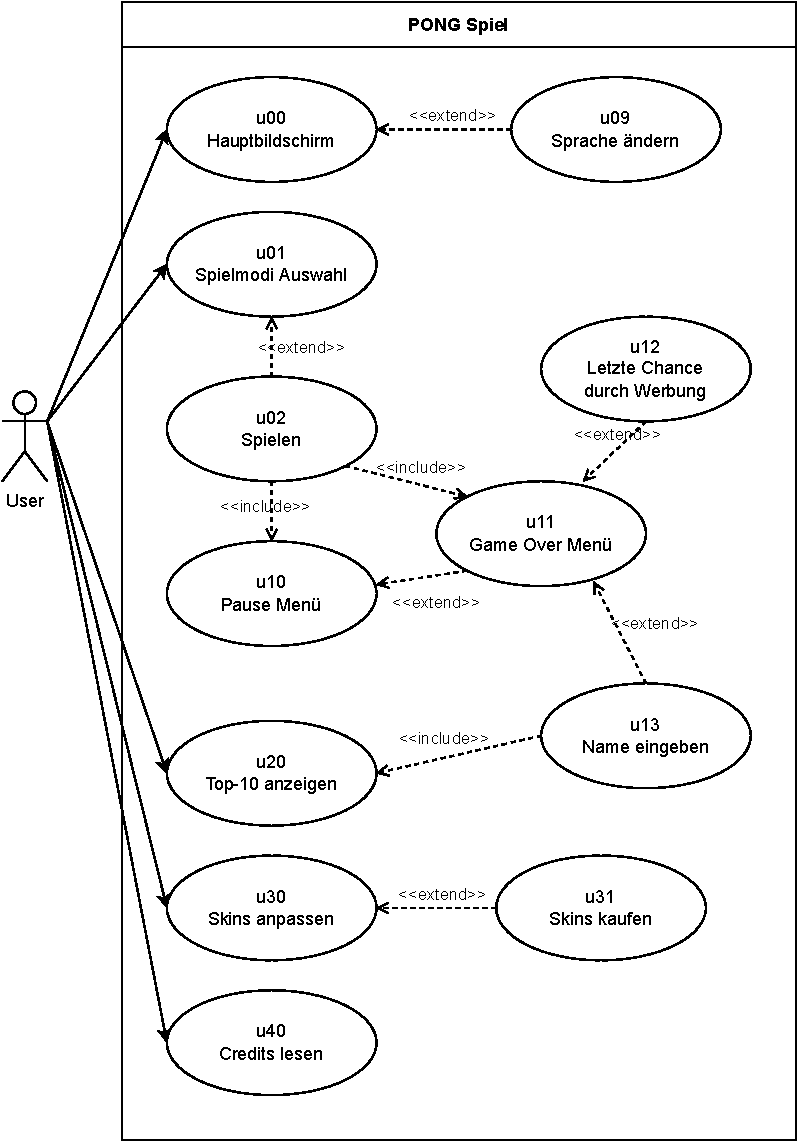
\includegraphics[width=\textwidth]{diagramme/pdf/UML-UseCase.pdf}
    \caption{Use Case Diagramm - Pong}
    \label{fig:use-case-diagram}
\end{figure}
